% 202010??
\documentclass[env.tex]{subfiles}
\begin{document}

\subsection{Temperature-standardisation}
The procedure included two parts.  Parameter values collected from literature were temperature-tagged.  For parameters with limited data, most of the reported experiments were done under \temp.  This study chose 23\textsuperscript{o}C as the standard temperature reference for the model; growth rate data was re-standardised to this temperature using Arrhenius Equation.

\begin{equation}
    A = A_0e^{-\dfrac{E_a}{k(T_C+273.15)}}
    \label{arrEq}
\end{equation}

which $A$ is the unit-standardised rate in data and $A_0$ is the standardisation constant with the same unit, $E_a$ is the activation energy with unit eV, $k$ is Boltzmann constant from Scipy (v1.4.1) package under unit eV/K and $T_C$ is the temperature of the organism measured from the data with unit (\textsuperscript{o}C).

Activation energies for phytoplanktons and \bac\ are 0.32eV and 0.66eV respectively\autocite{regaudie2012temperature}.  Standardised rate unit in data was ``sec\textsuperscript{-1}"; it was re-standardised to ``\dayU" for this study (Fig.\ref{f:A0}).

\begin{figure}[H]
    \centering
    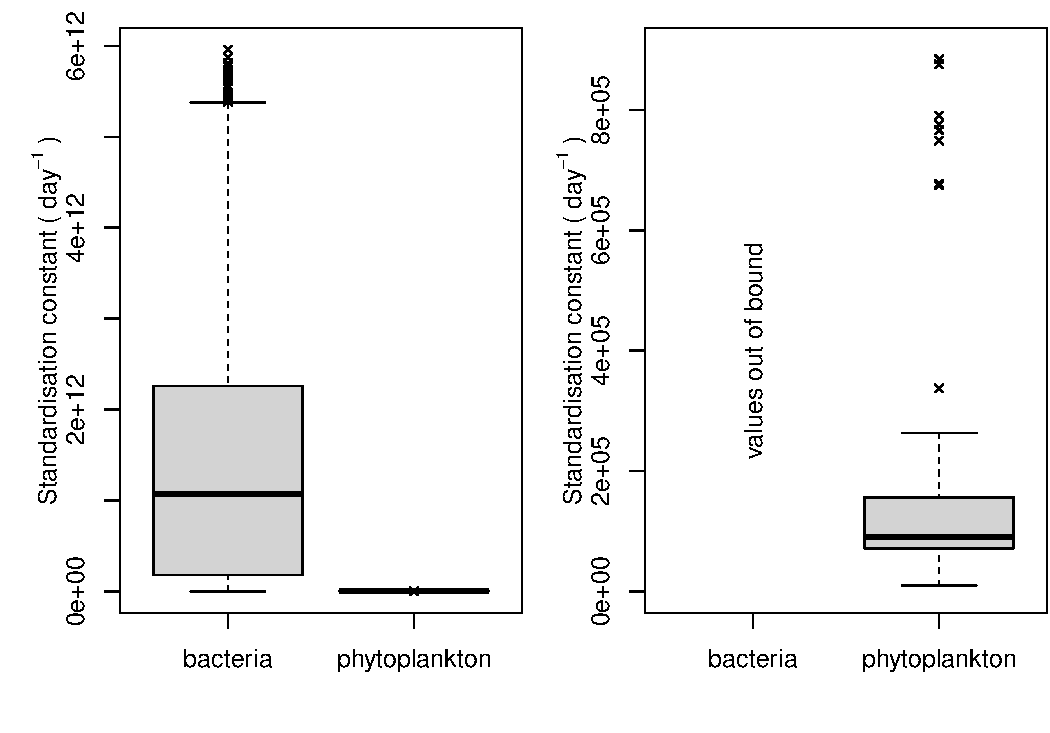
\includegraphics[width=.7\linewidth]{../result/stdCst.pdf}
    \caption[Boxplot of standardised $A_0$]{Boxplots of $A_0$ for \phy\ and \bac\ with unit ``\dayU"}
    \label{f:A0}
\end{figure}

\subsection{\Phy\ growth rates data wrangling}
Growth rate data was obtained from ``BioTrait" database\autocite{della2013thermal}.  Six filters were applied to extract published aquatic microbial \phy\ $P$ or \bac\ $B$ species entries which were identified to species level.  The matched data set was further filtered to eliminate entries reported no growth to facilitate the temperature standardisation step mentioned in the previous section.

Percentage range was calculated by the deviation of rate extremes from the mean.  The parameter range was calculated by mean of the standardised \phy\ growth rates $\pm$ percentage range of its own.  This range was chosen to construct the percentage ranges for data-deficient (min data entries of 5) rate parameters.

\subsection{\Bac\ clearance rates data wrangling}
``BioTrait" data \autocite{della2013thermal} was filtered by the same criteria as \phy\ but with \bac.  Temperature-standardised growth rate data in unit \dayU\ however was not directly applicable due to the disagreement of units (unit in data: \dayU; unit for $\gB$: \denI).  Clearance rate for microbes were also technically unfeasible to measure.  Yet these two quantities were linearly-related:

\begin{equation}
    \text{[clearance]} \times \text{[resource density]} = \text{[growth]}
    \label{eq:gB}
\end{equation}

Temperature-standardised \bac l growth rates were therefore divided by an arbitrary density (10 was used in this study) to resolve the unit issue.  The arbitrary density was decided in order to make resultant ranges of \phy\ and \bac\ growth rate comparable.  The comparability was according to the metabolism rate similarity between similar body sized organisms proposed by the Metabolic Theory of Ecology \autocite{brown2004toward}.

Percentage range of $\gB$ was deduced using its own data following the same calculation method as $\gP$.

\subsection{Parameter ranges for intraspecific interference of \phy\ and death rate of \bac}
There were three data entries for $\aP$ \autocite{de2007biofixation} and one data entry for $\mB$ \autocite{cochran1988estimation}.  To overcome the data deficiency issue, percentage range of $\gP$ was used as the reference range to construct the parameter ranges for $\aP$ and $\mB$.

Note that $\aP$ data was recorded under experimental temperature 30\textsuperscript{o}C \autocite{de2007biofixation}.  Although there was a temperature mismatch, these data were still used because of no other available data.  The resultant parameter range was assumed covering possible parameter values in \temp.

\subsection{Non-respired carbon fraction for \phy\ data wrangling}
Data for $\ePR$ was available in the form of linear functions in \autocite{j1989respiration}.  These functions were temperature-tagged functions of respiration rates (y-axis) based on growth rates (x-axis).  Six linear functions were within the temperature range of \temp, so only the intercepts and slope values of these graphs were collected.

The non-respired fraction of carbon ($n(R')$) was deduced using the temperature-standardised \phy\ growth rates:

\begin{equation}
    n(R') = 1-n(R) = 1-\dfrac{[\text{intercept}]+[\text{slope}]\cdot\gP}{\gP}
    \label{ePReqn}
\end{equation}

Due to lack of matches of recorded species between growth rate data and linear functions, the pool of parameter values were calculated by pairing every available growth rate with every available intercept-slope couple.  Parameter range of $\ePR$ was calculated using the same method described above but the maximum value was capped at 1 because in the proposed model \phy\ cannot absorb organic carbon from the $C$ pool.  The percentage range for $\ePR$ was selected as the reference range for the ``fraction" category.

\subsection{Biomass assimilated carbon fraction for \phy\ data wrangling}
Temperature-tagged data for $\eP$ was available in two papers \autocite{j1989respiration,samejima1958heterotrophic}.  Both papers contained data matching the temperature range \temp.  Percentage range of $\eP$ was calculated and capped at 1 with the same reason as $\ePR$ of no reabsorption of organic carbon.

\subsection{Non-respired carbon fraction for bacterial decomposer parameter range calculation}
$\eBR$ was calculated from combining Fig.1b and glucose recovery rate values in the paper \autocite{cochran1988estimation} due to the limited available data.  In that figure a net 100mg of carbon originated from straw material was recovered per gram of straw at around 24-28 days (starting from day 0).  The recovery rate of carbon released by respiration originated from external glucose was 80\%.  Since in the environment carbon source was either external glucose or straw, the respired carbon fraction is $\dfrac{100\cdot10^{-3}}{28\cdot(1-0.8)}$ and the non-respired carbon fraction is (1-[respired fraction]).  This number was the mid-point of $\eBR$ parameter range, range limits were calculated according to the reference percentage range of $\ePR$.

\subsection{Biomass assimilated carbon fraction for bacterial parameter range calculation}
Parameter range of $\eB$ was calculated with the same method as $\eBR$ because only one data from  \autocite{cochran1988estimation} was available.

\subsection{Log yield flux comparisons between \phy-only and \pbs s (Fig.\ref{f:bacEffect} cont)}
\begin{figure}[H]
    \centering
    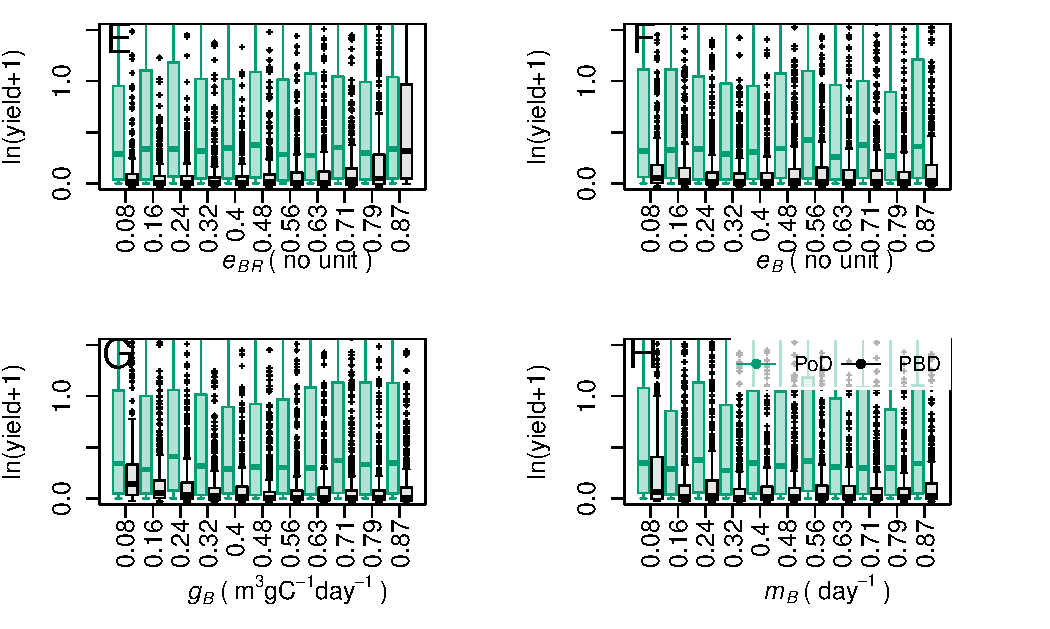
\includegraphics[width=.95\linewidth]{result/bacEff2.pdf}
    \caption[Log yield flux comparisons between feasible \phy-only and \pbs s (Fig.\ref{f:bacEffect} cont)]{Log yield flux comparisons between \phy-only and \pbs s on \bac\ parameters.  Note that medians were not significantly different for \PoN\ but significant for \PBN\ (Wilcox p$>$0.1 \& p$\ll$0.01 between extreme parameter values for \PoN\ and \PBN\ respectively).\lnExplain}
    \label{f:bacEffect2}
\end{figure}

\subsection{Log yield flux comparisons between \phy-only systems}
\begin{figure}[H]
    \centering
    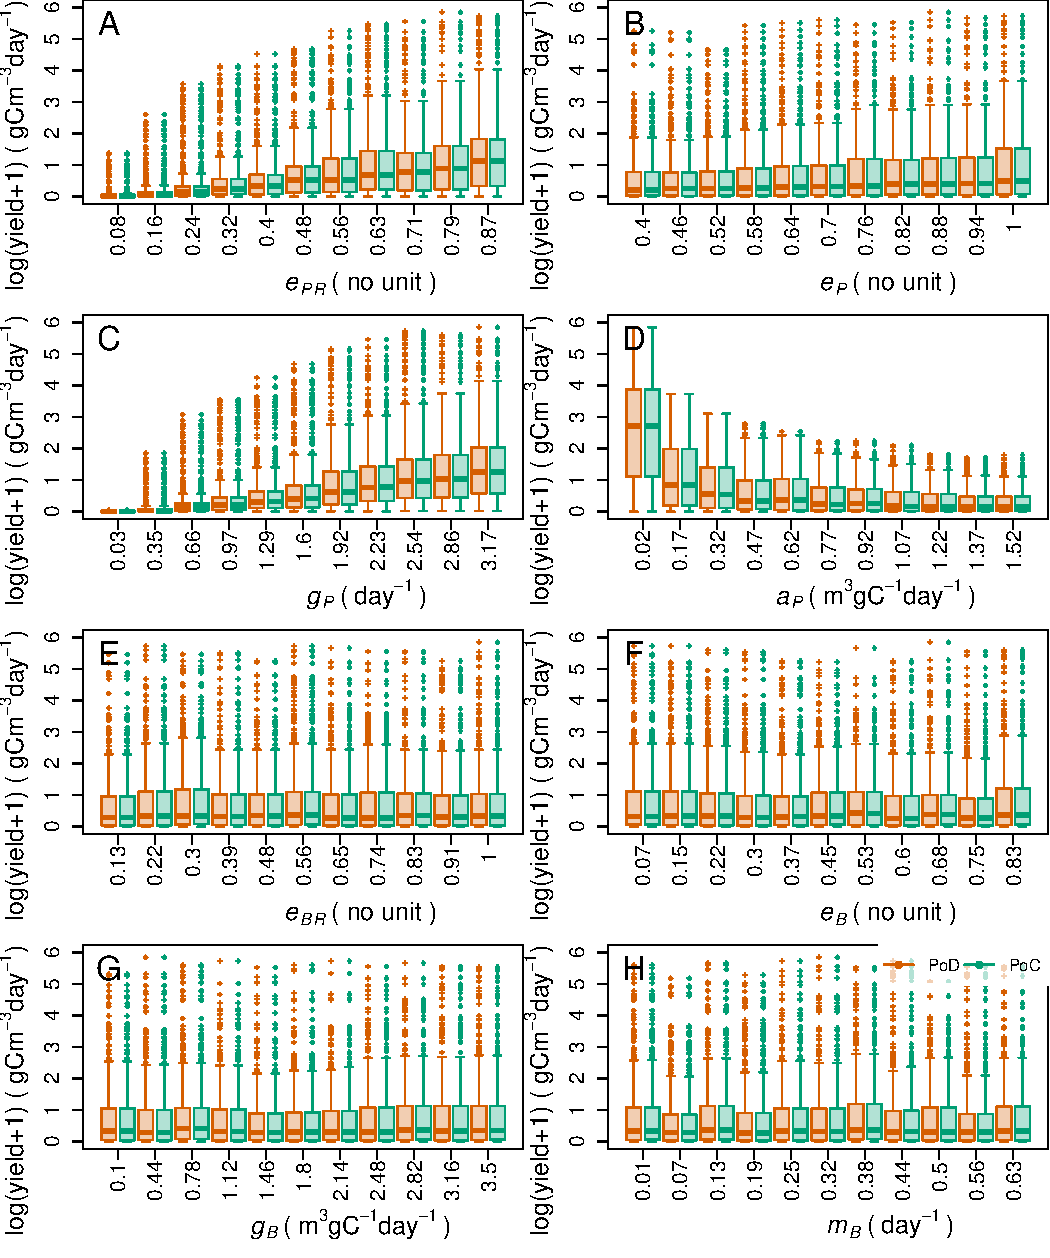
\includegraphics[width=.95\linewidth]{result/harvP.pdf}
    \caption[Log yield flux comparisons between \phy-only systems]{Log yield flux comparisons between \phy-only systems.  Note that distributions of \PoH\ and \PoN\ under optimised harvest interval/rate had no biological significance although with statistical significance (pairwise Wilcox p$\ll$0.01).  Also note that only \phy\ parameters had significant influence across respective parameter ranges (Wilcox p$\ll$0.01 between extreme parameter values in \textbf{(A)}, \textbf{(B)}, \textbf{(C)} and \textbf{(D)}.)\lnExplain}
    \label{f:harvPo}
\end{figure}

\end{document}